\skiptooddpage \section[Elhagyás, összehúzás,
  összeg,reprezentálhatóság]{Elhagyás és összehúzás. T test felett reprezentálhatóság.
  Matroidok direkt összege és összefüggősége.}


Legyen $M=(E,F)$ matroidon $X \subseteq E$ halmazra definiáljuk a következő
műveleteket:
\begin{description}
	\item[elhagyás] az $M \setminus X=(E-X, F \setminus Y)$, ahol $F \backslash
		      Y=\{Y\subseteq E-X, Y \in F\}$ (tehát az új matroidot úgy kapjuk, hogy
	      alaphalmazból elhagyjuk az $X$--beli elemeket és a halmazrendszerből meg azon
	      elemeket amelybe ezek részt vesznek).
	\item[összehuzás]  az $M / X=(E-X, F / X)$, ahol az $M/X$ rangfüggvénye felírható
	      $r(Y)=r(X \cup Y) - r(X), Y \in  E-X$ alakban (ha kivesszük az alaphalmazból az
	      összehúzott elemeket az új alaphalmaz -- $Y$ -- rangja egyenlő a teljes kezdeti alaphalmaz
	      -- $X \cup Y = E$-- és kivett alaphalmaz különbségével).
\end{description}

\begin{figure}[htbp]
	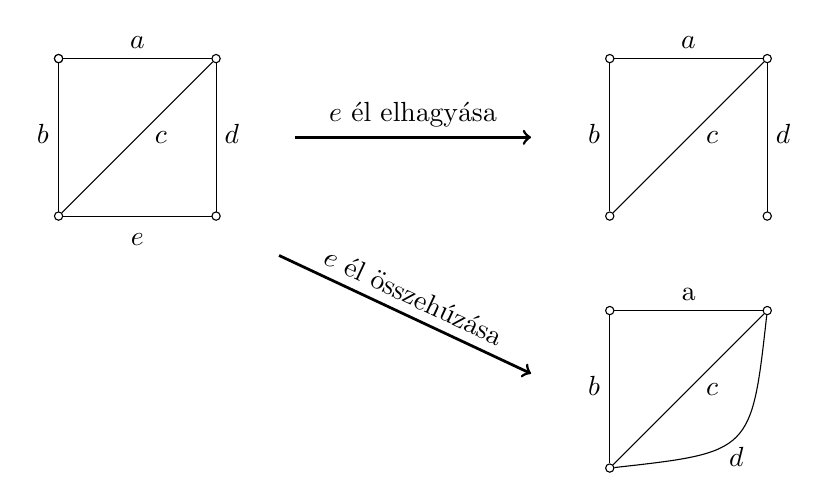
\begin{tikzpicture}
		\tikzstyle{vertex}=[draw,circle,fill=white,minimum size=3pt, inner sep=0pt]
		\begin{scope}
			\draw (0,0) node[vertex] (1){} -- ++(2cm,0) node[vertex](2){}
			-- ++(-90:2cm) node[vertex](3){}
			-- ++(-180:2cm) node[vertex](4){}
			-- ++(-270:2cm) node[vertex](5){};
			\draw (2) -- (4);
			\draw (1,0.2) node{$a$};
			\draw (-0.2,-1.0) node[anchor=mid]{$b$};
			\draw (1.3,-1.0) node[anchor=mid]{$c$};
			\draw (2.2,-1.0) node[anchor=mid]{$d$};
			\draw (1,-2.3) node{$e$};
		\end{scope}

		\begin{scope}[line width=1pt,join=miter]
			\draw[->] (3,-1) -- (6,-1) node[sloped, above, midway] {$e$ él elhagyása};
		\end{scope}

		\begin{scope}[xshift=7cm]
			\draw (0,0) node[vertex] (1a){}
			-- ++(2cm,0) node[vertex](2a){}
			-- ++(-90:2cm) node[vertex](3a){};
			\draw (0,-2) node[vertex](4a){};
			\draw (4a) -- (1a);
			\draw (2a) -- (4a);

			\draw (1,0.2) node{$a$};
			\draw (-0.2,-1.0) node[anchor=mid]{$b$};
			\draw (1.3,-1.0) node[anchor=mid]{$c$};
			\draw (2.2,-1.0) node[anchor=mid]{$d$};
		\end{scope}

		\begin{scope}[line width=1pt,join=miter]
			\draw[->] (2.8,-2.5) -- (6,-4) node[midway, sloped, above] {$e$ él összehúzása};
		\end{scope}
		%		\draw (0,0) node[vertex] (1){} 	.. controls ++(288:1cm) and ++(0:1cm) .. (1){};

		\begin{scope}[xshift=7cm, yshift=-3.2cm]
			\draw (0,0) node[vertex] (1b){}
			-- ++(2cm,0) node[vertex](2b){};
			\draw (0,-2) node[vertex](4b){};
			\draw (4b) -- (1b);
			\draw (2b) -- (4b);
			\draw (2b) .. controls (1.8,-1.8) .. (4b) node[midway, below]{$d$};

			\draw (1,0.2) node{a};
			\draw (-0.2,-1.0) node[anchor=mid]{$b$};
			\draw (1.3,-1.0) node[anchor=mid]{$c$};
		\end{scope}
	\end{tikzpicture}
	\caption{Elhagyás és összehúzás művelet grafikus
		matroidban}\label{fig:ElhagyOssze}
\end{figure}


Az elhagyás és az összehúzás műveletek prioritása azonos, tehát felcserélhető.
$M$ matroid \emph{minora} annak egy elhagyás és összehúzás sorozata. Bármely matroid minora előáll
$N=(M \setminus A) / B$ alakban, ahol $A$ és $B$ diszjunkt halmazok.

\emph{Az elhagyás és az összehúzás duális művelet: $\begin{cases}
			M^*/X=(M \setminus X)^*, \\
			M^* \setminus X = (M / X)^*.
		\end{cases}$}

A bizonyításhoz elég az elsőt belátni, mert ha az igaz, mindkét oldal duálisát
véve és $M$ helyet $M^*$--ra alkalmazva azt következik a második kijelentés.
Tudjuk tehát, hogy az duális matroid összehúzásának ($M^*/X$) rangfüggvénye
(legyen ez $r_1$):

\begin{align*}
	r_1(Y) & =\underbrace{r^*(X \cup Y)}_{|X \cup Y| + r(E-X-Y) - r(E)} -
	\underbrace{r^*(X)}_{|X| + r(E-X) - r(E)}                             \\
	       & = |Y| + r(E-X-Y) - r(E-X)
\end{align*}

Ugyanakkor a matroidból X elhagyásával ($M^*/X$) a rangfüggvény ($r_2$):

\[ r_2(Y) = |Y| + r(T-Y) - r(T),\] ahol $T = E-X$ az $M\setminus X$ matroid
alaphalmazza. Látjuk, hogy $r_1(Y)=r_2(Y)\Rightarrow$ minden $Y$--ra a a két
matroid megegyezik, s ezzel bizonyitásunk teljes.

\begin{description}
	\item[direkt összeg] $\begin{rcases}
			      M_1=(E_1,F_1) \mbox{ matroid}, \\
			      M_2=(E_2,F_2) \mbox{ matroid}, \\
			      E_1, E_2 \mbox{ diszjunkt, nem üres}\end{rcases} N = M_1+ M_2$ alaphalmaza
	      $E_1 \cup E_2$, és $X \subseteq E_1 \cup E_2$ halmaz akkor független a direkt
	      összegben, ha $X \cap E_1$ független $M_1$--ben és $X \cap E_2$ független
	      $M_2$--ben.
	\item[egy matroid \emph{összefüggő}] ha nem áll elő matroidok direkt
	      összegeként. A grafikus matroid akkor összefüggő, ha a gráf kétszeresen
	      összefüggő.
	\item[$M=(E,F)$ reprezentálható] T test felett, ha bármely elem az alaphalmazból
	      $T$ feletti vektor.
	\item[$M$ matroid koordinázható]T test felett, ha létezik olyan mátrix, amelynek oszlopai
	      $T$ felett vektorok, és az ezek által meghatározott lináris matroid izomorf
	      $M$--el.
\end{description}

Bármely $r=r(E), n=|E|$ matroidra létezik $A \in \mathbb{M}_{r\times n}$ mátrix
amellyel leírható $M=(E,F)$ matroid (és a mátrix sorai lineárisan függetlenek).
Az $A$ mátrix megalkotásához $r$ sorra van szükség, ha a matroid több elemet
tartalmaz válasszunk ki $r$ lineárisan függetlent. Ekkor a jobb oldali alakra
hozható $A$ mátrix, ettől még ugyanazt a matroidot koordinázza:

\[
	\overbrace{
		\begin{array}{|lcr|}
			\hline
			1      & \cdots            & r \\
			\vdots & \mbox{det} \neq 0 &   \\
			r      &                   &   \\
			\hline
		\end{array}}^{\mbox{egység alaká alakít}}
	\cdot~
	\begin{array}{|lcr|}
		\hline
		1      & \cdots & n \\
		\vdots & A      &   \\
		r      &        &   \\
		\hline
	\end{array}
	=
	\begin{array}{|lcr|}
		\hline
		1      & \cdots & n \\
		\vdots & B      &   \\
		r      &        &   \\
		\hline
	\end{array}
	=
	\begin{array}{|lcr|lcr|}
		\hline
		1      & \cdots & r & 1      & \cdots & n-r \\
		\vdots & I_r    &   & \vdots & A'     &     \\
		r      &        &   & r      &        &     \\
		\hline
	\end{array}
\]

\emph{Ha $M=(E,F)$ matroid reprezentálható $T$ test felett akkor a duálisa ($M*$) is.}

A bizonyitáshoz hozzuk a matroid mátrixát olyan alakra, hogy a mátrix bal
oldalán egy egységmátrix alakuljon ki. Legyen ennek $r$ sora, ekkor $E_r$ egységmátrix
M egy bázisa, míg $A_0$ oszlopai a többi elemek. Megpróbáljuk belátni, hogy $A'=(-A_0^T|E_{n-r})$
is reprezentálja a duális matroidot.

\[
	M=
	\begin{array}{|cc|c|c|rc|}
		\hline
		1      & 0      & \multicolumn{1}{>{\columncolor{lightgray}}l}{\color{black}0}    & \multicolumn{1}{>{\columncolor{gray}}l}{\color{white}C}     &     & \\
		\vdots & 1      & \multicolumn{1}{>{\columncolor{lightgray}}l}{\color{black}0}    & \multicolumn{1}{>{\columncolor{gray}}l}{\color{white}}      & A_0 & \\
		0      & \cdots & \multicolumn{1}{>{\columncolor{ColorGreyish}}l}{\color{black}1} & \multicolumn{1}{>{\columncolor{lightgray}}l}{\color{black}} &     & \\
		\hline
	\end{array}
	\Rightarrow
	M^*=
	\begin{array}{|c|c|cc|lcr|}
		\hline
		\multicolumn{1}{>{\columncolor{gray}}l}{\color{white}}           &                                     & 1                                     &                                          & \multicolumn{1}{>{\columncolor{lightgray}}l}{\color{black}0}    & \multicolumn{2}{>{\columncolor{lightgray}}l}{\color{black}}                                                                       \\
		\multicolumn{1}{>{\columncolor{gray}}l}{\color{white}-C^T}       &                                     &                                       & 1                                        & \multicolumn{2}{>{\columncolor{lightgray}}l}{\color{black}}     & \multicolumn{1}{>{\columncolor{lightgray}}l}{\color{black}0}                                                                      \\
		\cline{1-1} \cline{5-7}
		\multicolumn{1}{>{\columncolor{lightgray}}l}{\color{black}}      &                                     &                                       &                                          & \multicolumn{1}{>{\columncolor{ColorGreyish}}l}{\color{black}1} & \multicolumn{1}{>{\columncolor{ColorGreyish}}l}{\color{black}}  & \multicolumn{1}{>{\columncolor{ColorGreyish}}l}{\color{black}0} \\
		\multicolumn{1}{>{\columncolor{lightgray}}l}{\color{black}A_0^T} &                                     &                                       &                                          & \multicolumn{1}{>{\columncolor{ColorGreyish}}l}{\color{black}}  & \multicolumn{1}{>{\columncolor{ColorGreyish}}l}{\color{black}1} & \multicolumn{1}{>{\columncolor{ColorGreyish}}l}{\color{black}}  \\
		\multicolumn{1}{>{\columncolor{lightgray}}l}{\color{black}}      &                                     &                                       &                                          & \multicolumn{1}{>{\columncolor{ColorGreyish}}l}{\color{black}0} & \multicolumn{1}{>{\columncolor{ColorGreyish}}l}{\color{black}}  & \multicolumn{1}{>{\columncolor{ColorGreyish}}l}{\color{black}1} \\ \hline
		\multicolumn{1}{c}{\mathsmaller{r-t}}                            & \multicolumn{1}{c}{\mathsmaller{t}} & \multicolumn{2}{c}{\mathsmaller{r-t}} & \multicolumn{3}{c}{\mathsmaller{n-2r+t}}
	\end{array}
\]

$M$ matroid és a duálisának a mátrixa természetes módon megfelelhetőek
egymásnak, az ábrán balról jobbra az oszlopcsoportok megfelelnek egymásnak.
Válaszunk ki az $M$ valamely bázisának megfelelő részmátrixot $A$--ban.
Feltehető, hogy ennek első $t$ oszlopa éppen $E_r$ utolsó $t$ oszlopa, míg a
maradék $r-t$ oszlop $A_0$ első $r-t$ oszlopa. Ennek a mátrixnak determinánsa
akkor nem nulla, ha $C$ determinánsa nem nulla. Mivel $B$ bázis, ezért $C$ nem
szinguláris.

$B^*=E-B$ elemeinek $A'$--ben az a mátrix felel meg, amely első $r-t$ oszlopa
$-A_0^T$, a többi pedig $E_{n-r}$ utolsó $n-2r+t$ oszlopa. Ennek a felső
blokk--háromszög mátrix determinánsa akkor nem nulla, ha $-C^T$ determinánsa nem
nulla.  Azaz, hogy $C$ nem szinguláris. Tehát a bázis komplementere is bázis, és
fordítva, és ezért $A'$ valóban a duálist reprezentálja.
